\documentclass[UTF8,a4paper,11pt,fontset=fandol]{ctexart}
\usepackage[margin=25mm,headheight=15pt]{geometry}
\usepackage{amsmath,amssymb,amsthm,mathtools,booktabs,array,graphicx}
\usepackage{enumitem,fancyhdr,xcolor,hyperref}
\usepackage{tikz}
\hypersetup{unicode=true,colorlinks=true,linkcolor=blue!40!black,citecolor=blue!40!black,urlcolor=blue!40!black,
pdftitle={三行矩形多米诺铺法的对称计数及奇数高度推广},
pdfauthor={Shiqi Liu},pdfsubject={多米诺铺法的对称轨道计数},
pdfkeywords={domino tilings, A232622, Burnside, generating functions, Lean}}
\newtheorem{theorem}{定理}[section]
\newtheorem{lemma}[theorem]{引理}
\newtheorem{proposition}[theorem]{命题}
\newtheorem{corollary}[theorem]{推论}
\theoremstyle{definition}
\newtheorem{definition}[theorem]{定义}
\theoremstyle{remark}
\newtheorem{remark}[theorem]{注}
\renewcommand{\proofname}{证明}
\newcommand{\Fix}{\operatorname{Fix}}
\newcommand{\Stab}{\operatorname{Stab}}
\newcommand{\rev}{\operatorname{rev}}
\newcommand{\one}{\boldsymbol{1}}
\newcommand{\evec}{e_0}
\newcommand{\trans}{\mathsf T}
\numberwithin{equation}{section}
\setlength{\parskip}{0.3em}
\setlist{nosep}
\allowdisplaybreaks[2]
\pagestyle{fancy}
\fancyhf{}
\fancyhead[L]{\small 三行矩形多米诺铺法的对称计数}
\fancyhead[R]{\small Shiqi Liu}
\fancyfoot[C]{\thepage}
\title{\bfseries 三行矩形多米诺铺法的对称计数\\[4pt]
\large 基本块、半棋盘与奇数高度推广}
\author{Shiqi Liu}
\date{2026 年 10 月 25 日\quad 版本 2.1}
\begin{document}
\maketitle
\begin{abstract}
本文研究无标号多米诺对三行、偶数列矩形的全部铺法在旋转和反射下的轨道计数。
首先利用完整的列切口转移规则，将铺法唯一分解为不可竖切基本块，并把对称作用转化为字母对合和字的倒序。
由此证明 Mathar 提出的、收录于 OEIS A232622 的生成函数公式，并导出七阶递推及其全部初值。
其次建立半棋盘与对称固定铺法之间的双射，以两维递推重新得到三行公式，
并确定各精确稳定子类型及其渐近比例。
同一半棋盘方法给出任意固定奇数高度的轨道生成函数矩阵表达式及有理性；
五行情形进一步得到显式有理式、十四阶递推和六维多项式证书。
三行主计数定理另沿半棋盘路线在 Lean 中完成形式化验证，其系数直接定义为实际铺法轨道的基数。
文中明确区分形式化覆盖范围、一般演绎证明与有限计算检查，并提供源码及复现材料。
\end{abstract}
\noindent\textbf{关键词：} 多米诺铺法；Burnside 引理；生成函数；转移矩阵；对称轨道

\section{问题、记号与主要结果}
\label{sec:intro}

\subsection{计数对象与文献背景}
对整数 $n\ge1$，令 $\mathcal T_n$ 为 $3\times2n$ 单位格矩形的全部多米诺铺法。
每块砖覆盖两个共边相邻的格子，允许横放或竖放；铺法是这些无序格对的集合，
砖不带标号，不重叠、不留空，也不施加 tatami 条件。
行号从上到下为 $r=1,2,3$，列号从左到右为 $c=1,\ldots,2n$。定义
\[
 h(r,c)=(4-r,c),\qquad v(r,c)=(r,2n+1-c),\qquad \rho=hv.
\]
记 $G=\{e,h,v,\rho\}$，其中 $h$ 为上下反射，$v$ 为左右反射，$\rho$ 为半周旋转。
因为 $3\ne2n$，$G$ 是保持该矩形的完整平面等距对称群。
令 $a(n)=|\mathcal T_n/G|$。对 $n=0$，规定只有一个空铺法，四个抽象群元素均固定它，
故 $a(0)=1$。此约定允许群作用不忠实。

Mathar \cite{mathar2013} 的表 10 和 Conjecture 6 给出三行对称轨道计数及其猜想生成函数；
OEIS A232622 \cite{oeis} 列有等价的有理式和七阶递推。
2026 年 10 月 25 日核查时，OEIS 页面仍保留猜想标签；
这一页面状态不构成对全部既有文献或问题开放状态的判定。
本文的目标是给出这组公式的自足推导，并整理其对称细化与奇数高度推广。

固定宽度铺法的有限状态方法是已有工具。Mathar \cite{mathar2014} 的第 2.1--2.3 节
讨论了三行普通铺法和不可竖切块的生成函数。
DeFord \cite[定理 6.1]{deford} 研究了固定高度矩形在对称作用下的铺法计数，
给出此类序列满足常系数线性递推的一般框架。
因此，对称轨道生成函数的有理性本身已有文献基础。
本文重新证明所需块分类，补充反射和旋转在基本块字上的作用，
并用另一种半棋盘双射处理固定点。本文不以文献中的目标猜想、
有限数列或程序输出作为一般证明的前提。
本文着重给出三行目标公式的两条自足推导、精确对称类型、
奇数高度的明确边界向量及五行有限代数证书。
三行半棋盘路线还提供从实际铺法定义到主生成函数的 Lean 证明；
具体公式及证明方法的文献优先权仍待系统核查。

\subsection{主定理}
四类固定点数分别记为
\[
 d_n=|\mathcal T_n|,\quad h_n=|\Fix(h)|,\quad
 v_n=|\Fix(v)|,\quad r_n=|\Fix(\rho)|,
\]
其以半长度 $n$ 为指数的普通生成函数记为 $D,H,V,R$。
除渐近分析外，本文所有生成函数都在 $\mathbb Q[[x]]$ 中解释。

\paragraph{下标与计数的阅读约定。}
生成函数指数 $n$ 始终记录完整棋盘宽度 $2n$ 的一半。
第 \ref{sec:half} 节的 $q_w(S)$ 使用实际部分棋盘宽度 $w$，
而归纳指标 $j$ 将宽度写为 $2j$ 与 $2j+1$。
因此 $\alpha_j=q_{2j}(\varnothing)=d_j$，
$\beta_j=q_{2j}(\{1,2\})$ 只计一个末端状态。
完整状态转移使用行向量，式 \eqref{eq:two-dimensional} 的二维压缩使用列向量。

\begin{theorem}[三行对称轨道的生成函数]\label{thm:main}
对上述全部铺法，有
\begin{equation}\label{eq:main}
 A(x):=\sum_{n\ge0}a(n)x^n
 =\frac{1-3x-4x^2+10x^3-4x^5+x^6}
 {(1-x)(1-4x+x^2)(1-4x^2+x^4)}.
\end{equation}
相应递推为
\begin{equation}\label{eq:recurrence}
\begin{split}
a(n)={}&5a(n-1)-a(n-2)-19a(n-3)+19a(n-4)\\
       &+a(n-5)-5a(n-6)+a(n-7),\qquad n\ge7,
\end{split}
\end{equation}
初值为 $(a(0),\ldots,a(6))=(1,2,5,14,46,156,561)$。
\end{theorem}

式 \eqref{eq:main} 分子、分母同乘 $-1$ 即得到 OEIS 所列形式。
第 \ref{sec:blocks} 节给出基本块证明；
第 \ref{sec:half} 节用半棋盘方法重新推导四类固定点数。
第 \ref{sec:types} 节确定精确稳定子并研究对称比例；
第 \ref{sec:odd} 节推广到任意固定奇数高度，
第 \ref{sec:five} 节给出五行显式实例。五行计算所需的全部小矩阵在附录中列出。
第 \ref{sec:formalization} 节说明三行主定理的形式化对应及验证边界。

\begin{lemma}[轨道平均公式]\label{lem:burnside}
对每个 $n\ge0$，
\begin{equation}\label{eq:burnside}
 a(n)=\frac{d_n+h_n+v_n+r_n}{4}.
\end{equation}
\end{lemma}
\begin{proof}
双重计数集合 $\{(g,T):g\in G,\ T\in\mathcal T_n,\ gT=T\}$ 得
\[
 \sum_{g\in G}|\Fix(g)|=\sum_{T\in\mathcal T_n}|\Stab(T)|.
\]
轨道稳定子公式表明，一个轨道 $O$ 对右边的贡献为
$|O|\cdot4/|O|=4$，故得所需等式。
这也是 Burnside 引理 \cite[第 7 章，Lemma 7.2]{stanley} 在本问题的应用。
上述计数不要求作用忠实，因而包含空棋盘。
\end{proof}

\section{基本块分解与第一种证明}\label{sec:blocks}

\subsection{列切口的完整状态规则}
先考虑任意宽度 $w$ 的三行棋盘。在第 $j$ 列与第 $j+1$ 列之间记
$S_j\subseteq\{1,2,3\}$ 为被水平砖跨越的行集合，端点取
$S_0=S_w=\varnothing$。
若一列的输入和输出状态分别为 $p,q$，则合法的充要条件为
\begin{equation}\label{eq:local3}
 p\cap q=\varnothing,\qquad
 \{1,2,3\}\setminus(p\cup q)\in
 \{\varnothing,\{1,2\},\{2,3\}\}.
\end{equation}
理由是输入行的格已被左来的砖占用，输出行用于向右的砖，其余格必须在本列用竖直砖配对。
每个合法转移的本列填充唯一。全部转移见表 \ref{tab:states}。

\begin{table}[htbp]
\centering
\caption{三行的完整列状态转移。}\label{tab:states}
\begin{tabular}{cc@{\qquad}cc}
\toprule
输入 & 全部输出 & 输入 & 全部输出\\
\midrule
$\varnothing$ & $\{1\},\{3\},\{1,2,3\}$ &
$\{1,2\}$ & $\{3\}$\\
$\{1\}$ & $\varnothing,\{2,3\}$ &
$\{1,3\}$ & $\{2\}$\\
$\{2\}$ & $\{1,3\}$ &
$\{2,3\}$ & $\{1\}$\\
$\{3\}$ & $\varnothing,\{1,2\}$ &
$\{1,2,3\}$ & $\varnothing$\\
\bottomrule
\end{tabular}
\end{table}

\begin{lemma}\label{lem:path}
三行、$w$ 列的完整铺法与表 \ref{tab:states} 中长度为 $w$、
从空状态回到空状态的合法路径一一对应。
\end{lemma}
\begin{proof}
铺法唯一确定各切口状态。反过来，在每个切口状态指定的行放跨切口水平砖，
再在每列剩余行放唯一的竖直砖。式 \eqref{eq:local3} 保证同格不被两个水平砖重复使用，
且剩余格恰好被竖直砖覆盖。端点空状态排除越界砖。
两种构造互逆；$w=0$ 对应空路径。
\end{proof}

\subsection{首次回返路径与不可竖切块}
\begin{definition}
若一个内部竖直格线没有砖跨越，称它为断口。
非空完整铺法若没有内部断口，称为基本块。
\end{definition}

\begin{lemma}[基本块分类]\label{lem:blocks}
所有三行基本块恰为 $C$ 及 $A_k,B_k$（$k\ge1$）。
其中 $C$ 为宽 2 的三块水平砖；$A_k$ 宽 $2k$，由下列砖组成：
\begin{enumerate}
\item 第 1 列和第 $2k$ 列各放一块覆盖第 1、2 行的竖直砖；
\item 第 3 行按列对 $(2j-1,2j)$ 铺满，$1\le j\le k$；
\item 第 1、2 行内部各按列对 $(2j,2j+1)$ 铺满，$1\le j<k$。
\end{enumerate}
最后令 $B_k=h(A_k)$。
\end{lemma}
\begin{proof}
基本块对应空状态的首次回返路径。从空状态出发只有三个分支。
若第一步到 $\{1,2,3\}$，下一步被迫回空状态，给出 $C$。
若第一步到 $\{3\}$，则在最终回空状态之前，
只能在 $\{3\}$ 与 $\{1,2\}$ 之间交替。路径恰为
\[
 \varnothing\longrightarrow\{3\}
 \longrightarrow
 \bigl(\{1,2\}\longrightarrow\{3\}\bigr)^{k-1}
 \longrightarrow\varnothing,\qquad k\ge1,
\]
这里括号内表示两步的重复，$k=1$ 时重复零次。
路径给出所述 $A_k$ 坐标。第一步到 $\{1\}$ 的分支
只能在 $\{1\},\{2,3\}$ 之间交替后回空状态，得到 $B_k$。
表 \ref{tab:states} 穷尽了这些分支的所有后继，因而无遗漏。
$A_k$ 的奇数内部切口由第 3 行水平砖跨越，
偶数内部切口由第 1、2 行水平砖跨越，故确实无断口；
$B_k$ 由反射得到同样性质。
首列的竖直砖位置区分 $A_k,B_k$，而 $C$ 无竖直砖，故无重计。
\end{proof}

\begin{figure}[htbp]
\centering
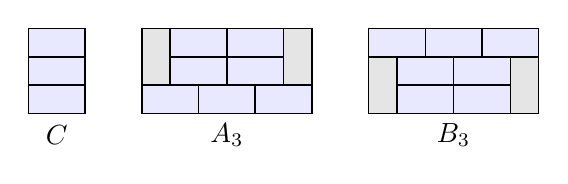
\begin{tikzpicture}[x=0.36cm,y=0.36cm,line width=0.55pt]
\begin{scope}
 \foreach \y in {0,1,2}{\draw[fill=blue!9] (0,\y) rectangle ++(2,1);}
 \node at (1,-0.75) {$C$};
\end{scope}
\begin{scope}[shift={(4,0)}]
 \draw[fill=gray!20] (0,1) rectangle (1,3);
 \draw[fill=gray!20] (5,1) rectangle (6,3);
 \foreach \x in {0,2,4}{\draw[fill=blue!9] (\x,0) rectangle ++(2,1);}
 \foreach \y in {1,2}{\foreach \x in {1,3}{\draw[fill=blue!9] (\x,\y) rectangle ++(2,1);}}
 \node at (3,-0.75) {$A_3$};
\end{scope}
\begin{scope}[shift={(12,0)}]
 \draw[fill=gray!20] (0,0) rectangle (1,2);
 \draw[fill=gray!20] (5,0) rectangle (6,2);
 \foreach \x in {0,2,4}{\draw[fill=blue!9] (\x,2) rectangle ++(2,1);}
 \foreach \y in {0,1}{\foreach \x in {1,3}{\draw[fill=blue!9] (\x,\y) rectangle ++(2,1);}}
 \node at (3,-0.75) {$B_3$};
\end{scope}
\end{tikzpicture}

\caption{三种基本块的代表 $C,A_3,B_3$。矩形边界表示实际砖界；图示不代替一般分类证明。}
\label{fig:blocks}
\end{figure}

\begin{lemma}[唯一块分解及对称作用]\label{lem:word}
每个完整三行铺法唯一对应基本块字母表
$\mathcal B=\{C\}\cup\{A_k,B_k:k\ge1\}$ 上的一个有限字。
令 $\sigma$ 固定 $C$，交换 $A_k$ 与 $B_k$，则字上的作用为
\begin{equation}\label{eq:word-action}
 h(W)=\sigma(W),\qquad v(W)=\rev(W),\qquad
 \rho(W)=\sigma(\rev(W)).
\end{equation}
\end{lemma}
\begin{proof}
沿全部断口切开，所得各段无内部断口，故由引理 \ref{lem:blocks} 都是基本块。
任何基本块分解的分界必须是断口，而且不能遗漏断口，
否则有一块内部仍可竖切。这证明唯一性。任意基本块字的拼接给出逆映射。

上下反射在各块内按定义施加 $\sigma$。每个基本块还都左右对称：
对 $A_k$，列反转 $c\mapsto2k+1-c$ 交换两端竖直砖，
将底行列对 $(2j-1,2j)$ 映为同类列对，
将上两行列对 $(2j,2j+1)$ 映为同类列对；
对应指标分别为 $k+1-j$ 和 $k-j$。$C$ 逐砖不变。
由于上下、左右反射交换，$B_k=h(A_k)$ 也左右对称。

全棋盘反射保持断口集合；上下反射保留块次序，
左右反射颠倒块次序。结合唯一分解即得 \eqref{eq:word-action}。
论证允许相邻块宽度不同。
\end{proof}

\subsection{固定字的生成函数}
给 $C$ 权 $x$，给 $A_k,B_k$ 权 $x^k$，权的指数为半长度。
基本块生成函数为
\begin{equation}\label{eq:F}
 F(x)=x+2\sum_{k\ge1}x^k=\frac{3x-x^2}{1-x}.
\end{equation}
由于 $F(0)=0$，每个次数只涉及有限多个字，形式求和合法。

\begin{proposition}\label{prop:fixed-gf}
四种固定点生成函数为
\begin{align}
D(x)&=\frac{1}{1-F(x)}=\frac{1-x}{1-4x+x^2},&
H(x)&=\frac{1}{1-x},\label{eq:DH}\\
V(x)&=(1+F(x))D(x^2)
 =\frac{1+3x+x^2-x^3}{1-4x^2+x^4},\label{eq:V}\\
R(x)&=(1+x)D(x^2)
 =\frac{1+x-x^2-x^3}{1-4x^2+x^4}.\label{eq:R}
\end{align}
\end{proposition}
\begin{proof}
普通铺法对应任意字，故 $D=\sum_{\ell\ge0}F^\ell$。
上下反射固定字的每个字母须由 $\sigma$ 固定，唯一选择为 $C$，
故 $H=\sum_{\ell\ge0}x^\ell$。

左右反射固定字是回文，唯一写为
$U\rev(U)$ 或 $Ub\rev(U)$，其中 $b$ 为任意基本块。
两侧的总权是左侧权的平方，所以左半字贡献 $D(x^2)$，
中间贡献 $1+F(x)$，得到 \eqref{eq:V}。

半周旋转固定字唯一写为
$U\sigma(\rev(U))$，或 $Ub\sigma(\rev(U))$ 且 $\sigma(b)=b$。
后一种情形只允许 $b=C$，故中心贡献 $1+x$。
这两类互斥，分解可逆，得到 \eqref{eq:R}。
中心基本块允许跨越几何中线；上述计数没有附加中线必须为断口的限制。
\end{proof}

\begin{proof}[定理 \ref{thm:main} 的第一种证明]
由引理 \ref{lem:burnside} 和命题 \ref{prop:fixed-gf}，
\begin{equation}\label{eq:average-rational}
 A(x)=\frac14\left[
 \frac{1-x}{1-4x+x^2}+\frac1{1-x}
 +\frac{2(1+2x-x^3)}{1-4x^2+x^4}\right].
\end{equation}
记 $P_3=1-4x+x^2$、$Q_3=1-4x^2+x^4$。
通分后分子为
\[
 \frac{(1-x)^2Q_3+P_3Q_3+
 2(1+2x-x^3)(1-x)P_3}{4}
 =1-3x-4x^2+10x^3-4x^5+x^6.
\]
这给出 \eqref{eq:main}。分母展开为
\[
 1-5x+x^2+19x^3-19x^4-x^5+5x^6-x^7.
\]
因分子次数为 6，比较次数 $n\ge7$ 的系数得到
\eqref{eq:recurrence}；比较次数 $0,\ldots,6$ 得到所述初值。
\end{proof}

Mathar \cite[式 (26)]{mathar2013} 以全列数为指数，故与本文比较应取
$\overline T(z,3)=A(z^2)$。将 $x=z^2$ 代入
\eqref{eq:average-rational}，第一项重排利用
$\tfrac18((1+z)^{-1}+(1-z)^{-1})=(4(1-z^2))^{-1}$，
即得到该文献的表达式。
Mathar \cite[式 (4)--(6)]{mathar2014} 的三行公式以砖数计次，
对应换元为 $z^3=x$。两种变量约定不可混用。

\section{半棋盘双射与第二种证明}\label{sec:half}
本节从局部覆盖重新构造计数，不使用基本块分类或回文公式。
为便于后续推广，先允许任意整数高度 $m\ge1$。

\subsection{带末端半块的部分铺法}
对 $j\ge1$ 和 $S\subseteq\{1,\ldots,m\}$，令 $\mathcal P_m(j,S)$ 为
$m\times j$ 棋盘的部分铺法：除末列行号属于 $S$ 的格外，所有格都由内部多米诺覆盖；
这些未覆盖格标记为向右伸出的半块，准备与右邻格配成水平砖。
$j=0$ 时只有 $S=\varnothing$ 的空对象。记 $q_j(S)=|\mathcal P_m(j,S)|$。

令 $T_m$ 的行列按所有行子集排列。定义
\begin{equation}\label{eq:Tm}
 T_m[p,q]=
 \begin{cases}
 1,&p\cap q=\varnothing,\text{ 且 }[m]\setminus(p\cup q)
       \text{ 的每个连续段均为偶长},\\
 0,&\text{否则}.
 \end{cases}
\end{equation}
这里 $[m]=\{1,\ldots,m\}$，空补集满足条件。
每段偶长剩余行的竖直配对唯一，因为端点只能与相邻格配对，
剥去此对后继续。奇长段无法配满。
因此 \eqref{eq:Tm} 恰好刻画加一列的合法转移。
放入指定水平砖和唯一竖直配对给出逆构造，故
\begin{equation}\label{eq:profile}
 q_j^{\trans}=\evec^{\trans}T_m^j,\qquad
 t_m(j)=\evec^{\trans}T_m^j\evec,
\end{equation}
其中 $\evec$ 是空状态的单位列向量，$t_m(j)$ 为完整 $m\times j$ 铺法数。
辅助定义 $T_0=(1)$、$t_0(j)=1$。

\subsection{对称固定铺法的边界条件}
记 $J(S)=\{m+1-r:r\in S\}$，$\one$ 为全 1 列向量，
$\chi_m(S)=1$ 当且仅当 $J(S)=S$。
用 $v_{m,n},r_{m,n}$ 表示 $m\times2n$ 的左右反射、半周旋转固定数。

\begin{lemma}[中线补全双射]\label{lem:half}
对 $m\ge1$ 和 $n\ge0$，
\begin{equation}\label{eq:half-fixed}
 v_{m,n}=\evec^{\trans}T_m^n\one,\qquad
 r_{m,n}=\evec^{\trans}T_m^n\chi_m.
\end{equation}
\end{lemma}
\begin{proof}
先设 $n\ge1$。任取 $P\in\mathcal P_m(n,S)$，
将内部砖左右反射到右半棋盘，然后对每个 $r\in S$
插入连接 $(r,n)$ 与 $(r,n+1)$ 的水平砖。
两半内部砖不相交，跨中线砖恰好补齐剩余格，
得到唯一的左右反射固定铺法。
反向限制到左半，切断跨中线砖，唯一恢复 $P,S$，
因此所有 $S$ 都可取，并有第一式。

对半周旋转，将左半内部砖旋转到右半后，右侧待补行集合为 $J(S)$。
跨中线砖必须水平，故能补全的充要条件是 $J(S)=S$。
条件满足时逐行插入跨中线砖，所得砖集合在半周旋转下保持不变；
限制到左半是逆操作，得到第二式。
条件的必要性也来自跨中线第 $r$ 行的砖必须有第 $m+1-r$ 行的旋转像。
$n=0$ 时只有空对象，两式均为 1。
\end{proof}

\begin{lemma}[奇数高度的上下反射]\label{lem:h-odd}
若 $m=2k+1$，$k\ge0$，则
\begin{equation}\label{eq:h-odd}
 h_{m,n}=t_k(2n).
\end{equation}
\end{lemma}
\begin{proof}
在上下反射固定铺法中，接触中央行的竖直砖会被映到另一块竖直砖，
两者在中央行重叠，因此不存在这样的砖。
中央行只能以唯一方式水平铺满。其上 $k$ 行必须自行铺满，
下方由其反射唯一确定。任意上方完整铺法都给出一个固定铺法，
限制回上方为逆操作。$k=0$ 与 $n=0$ 由空对象约定覆盖。
\end{proof}

\subsection{三行的两维递推}
对 $m=3$，由 \eqref{eq:Tm} 从空状态可达的状态恰为
$\varnothing,\{1\},\{3\},\{1,2\},\{2,3\},\{1,2,3\}$。
规则给出空集的输出为两个端点单集和全体集合；
$\{1\}$ 的输出为 $\varnothing,\{2,3\}$，
$\{3\}$ 的输出为 $\varnothing,\{1,2\}$，
其余三个状态的输出分别被迫为 $\{3\},\{1\},\varnothing$。
下面将状态支持与计数同时归纳。记
\[
 E=\{\varnothing,\{1,2\},\{2,3\}\},\qquad
 O=\{\{1\},\{3\},\{1,2,3\}\}.
\]
完整转移表表明，$E$ 的全部出口在 $O$，$O$ 的全部出口在 $E$，
没有通向剩余两个状态的出口。这只表示允许的转移交替，
不表示两集合间任意一对状态都有转移。

\paragraph{归纳命题与基例。}
对每个 $j\ge0$，$q_{2j}$ 的支持包含于 $E$，且
\[
 q_{2j}(\varnothing)=\alpha_j,\qquad
 q_{2j}(\{1,2\})=q_{2j}(\{2,3\})=\beta_j.
\]
这里 $\beta_j$ 计数一个指定状态，两种非空状态合计为 $2\beta_j$。
支持包含于 $E$ 不要求其中每个状态都有正计数。
零宽只有空对象，所以 $(\alpha_0,\beta_0)=(1,0)$，
两个非空状态的计数相等且均为零。

\paragraph{增加第一列。}
假设 $2j$ 列时命题成立。按目标状态的全部来源求和，得到
\[
\begin{aligned}
q_{2j+1}(\{1\})
 &=q_{2j}(\varnothing)+q_{2j}(\{2,3\})=\alpha_j+\beta_j,\\
q_{2j+1}(\{3\})
 &=q_{2j}(\varnothing)+q_{2j}(\{1,2\})=\alpha_j+\beta_j,\\
q_{2j+1}(\{1,2,3\})&=q_{2j}(\varnothing)=\alpha_j.
\end{aligned}
\]
其余状态计数为零，因为 $E$ 的出口已穷尽。
每条合法单列转移的局部补法唯一；反过来，移除新增列并切断跨越其左边界的水平砖，
可恢复唯一旧对象和输入状态。因此各来源不重不漏，求和时不需要额外乘数。

\paragraph{增加第二列。}
$O$ 中三个状态都能转入空集；只有 $\{3\}$ 能转入 $\{1,2\}$，
只有 $\{1\}$ 能转入 $\{2,3\}$。于是
\[
\begin{aligned}
q_{2j+2}(\varnothing)
 &=q_{2j+1}(\{1\})+q_{2j+1}(\{3\})+q_{2j+1}(\{1,2,3\})\\
 &=(\alpha_j+\beta_j)+(\alpha_j+\beta_j)+\alpha_j
   =3\alpha_j+2\beta_j,\\
q_{2j+2}(\{1,2\})&=q_{2j+1}(\{3\})=\alpha_j+\beta_j,\\
q_{2j+2}(\{2,3\})&=q_{2j+1}(\{1\})=\alpha_j+\beta_j.
\end{aligned}
\]
因 $O$ 的全部出口在 $E$，其余状态仍为零。
这同时证明下一偶数列的支持和两个非空状态的计数相等性，
从而完成对全部 $j\ge0$ 的归纳。最后写成列向量递推：
\begin{equation}\label{eq:two-dimensional}
 \binom{\alpha_{j+1}}{\beta_{j+1}}
 =\begin{pmatrix}3&2\\1&1\end{pmatrix}
 \binom{\alpha_j}{\beta_j},\qquad
 (\alpha_0,\beta_0)=(1,0).
\end{equation}

\paragraph{四个矩阵系数的含义。}
第一行计数到达空集的对象；第二行只计数到达 $\{1,2\}$ 的对象。
\begin{center}
\small
\begin{tabular}{cp{0.78\linewidth}}
\toprule
系数 & 两列接续的计数理由\\
\midrule
$3$ & 从空集经 $\{1\}$、$\{3\}$ 或 $\{1,2,3\}$ 回空集，共三条路径。\\
$2$ & 从 $\{1,2\}$ 和 $\{2,3\}$ 各有一条回空集的路径；两组来源各有 $\beta_j$ 个对象。\\
$1$ & 从空集经 $\{3\}$ 到 $\{1,2\}$，有且仅有一条路径。\\
$1$ & 从 $\{1,2\}$ 经 $\{3\}$ 回到自身；另一非空状态不能在两步到达此目标。\\
\bottomrule
\end{tabular}
\end{center}
特别地，系数 $2$ 不是说每个固定非空状态对象有两种回空接法。
例如 $(\alpha_1,\beta_1)=(3,1)$ 给出
$\alpha_2=(3+1)+(3+1)+3=11$、$\beta_2=3+1=4$。
这个实例用于解释已证明的归纳，不作为一般结论的依据。

\begin{proposition}\label{prop:parity}
设 $d_j=t_3(2j)$，则
\begin{equation}\label{eq:d-rec}
 d_0=1,\quad d_1=3,\quad d_{j+2}=4d_{j+1}-d_j\quad(j\ge0).
\end{equation}
三行固定点数满足
\begin{equation}\label{eq:parity-fixed}
 h_n=1,\quad r_{2j}=r_{2j+1}=d_j,\quad
 v_{2j}=d_{j+1}-2d_j,\quad v_{2j+1}=d_{j+1}.
\end{equation}
因此
\begin{equation}\label{eq:parity-orbits}
 a(2j)=\frac{d_{2j}+1+d_{j+1}-d_j}{4},\qquad
 a(2j+1)=\frac{d_{2j+1}+1+d_{j+1}+d_j}{4}.
\end{equation}
\end{proposition}
\begin{proof}
由 \eqref{eq:profile}，$d_j=\alpha_j$。
式 \eqref{eq:two-dimensional} 中的矩阵满足 $M^2-4M+I=0$，
从而得 \eqref{eq:d-rec}。
偶数步可达的 $J$-不变集合只有空集，
奇数步可达的 $J$-不变集合只有全三行集合，故引理 \ref{lem:half} 给出 $r$ 的两式。
对所有状态求和，偶数步得
$\alpha_j+2\beta_j=d_{j+1}-2d_j$，
奇数步得 $3\alpha_j+2\beta_j=d_{j+1}$。
引理 \ref{lem:h-odd} 给出 $h_n=t_1(2n)=1$。
最后代入轨道平均公式即得 \eqref{eq:parity-orbits}。
\end{proof}

\begin{proof}[定理 \ref{thm:main} 的第二种证明]
递推 \eqref{eq:d-rec} 给出 $D(x)=(1-x)/(1-4x+x^2)$。
对 \eqref{eq:parity-fixed} 分别求和可得
\[
 H(x)=\frac1{1-x},\quad R(x)=(1+x)D(x^2),\quad
 V(x)=(1+x)\frac{D(x^2)-1}{x^2}-2D(x^2).
\]
这里 $D(x^2)-1$ 可唯一写为 $x^2 E(x)$，
其中 $E(x)=\sum_{j\ge0}d_{j+1}x^{2j}$；上式的商表示这一系数移位，
并未将 $x$ 或 $x^2$ 当作形式幂级数环中的单位。
化简 $V$ 得到 \eqref{eq:V}，再用轨道平均公式即得
\eqref{eq:average-rational}，其通分和系数比较已在前文完整写出。
本次推导的组合前提仅为半棋盘双射和单列覆盖规则。
\end{proof}

\section{精确对称类型与渐近行为}\label{sec:types}

\begin{theorem}[精确稳定子分类]\label{thm:stabilizers}
对三行、$2n$ 列棋盘，各精确稳定子的铺法数和轨道数见表 \ref{tab:stabilizers}。
该表对所有 $n\ge0$ 成立。
\end{theorem}
\begin{table}[htbp]
\centering
\caption{三行铺法的全部精确稳定子类型。}\label{tab:stabilizers}
\begin{tabular}{cccc}
\toprule
精确稳定子 & 铺法数 & 轨道大小 & 轨道数\\
\midrule
$G$ & $1$ & $1$ & $1$\\
$\{e,h\}$ & $0$ & $2$ & $0$\\
$\{e,v\}$ & $v_n-1$ & $2$ & $(v_n-1)/2$\\
$\{e,\rho\}$ & $r_n-1$ & $2$ & $(r_n-1)/2$\\
$\{e\}$ & $d_n-v_n-r_n+1$ & $4$ & $(d_n-v_n-r_n+1)/4$\\
\bottomrule
\end{tabular}
\end{table}
\begin{proof}
引理 \ref{lem:h-odd} 表明唯一的上下反射固定铺法是三行各自水平铺满的铺法，
它同时被 $v,\rho$ 固定。
若铺法同时由任意两个不同的非恒等群元素固定，则也由它们的积固定，
因而由整个 $G$ 固定。故三种固定集的两两交集和三重交集都是上述单点。
于是只具 $v$ 对称的铺法有 $v_n-1$ 个，只具 $\rho$ 对称的有 $r_n-1$ 个，
只具 $h$ 对称的有零个；其余 $d_n-v_n-r_n+1$ 个的稳定子平凡。
群 $G$ 交换，同一轨道中的稳定子相同。各类除以轨道大小即得表中结果。
四元群的子群只有表中五种，故分类完整。
\end{proof}

例如 $n=8$ 时 $d_8=29681,v_8=265,r_8=153$。
共有 $7525$ 个轨道，其中 $7316$ 个稳定子平凡，
$132$ 个精确稳定子为 $\{e,v\}$，$76$ 个为 $\{e,\rho\}$，$1$ 个为 $G$。

\begin{theorem}[对称铺法的渐近比例]\label{thm:asym}
令 $\lambda=2+\sqrt3$。均匀选取一个有固定棋盘方向的普通铺法时，
其具有非平凡对称的概率 $p_n$ 满足
\begin{align}
 p_{2j}&\sim(\lambda-1)\lambda^{-j},&
 p_{2j+1}&\sim\frac{\lambda+1}{\lambda}\lambda^{-j}
 \quad(j\to\infty).\label{eq:prob-asym}
\end{align}
特别地，$p_n=O(\lambda^{-n/2})\to0$，并且
\begin{equation}\label{eq:orbit-asym}
 a(n)=\frac{d_n}{4}+O(\lambda^{n/2})
 \sim\frac{3+\sqrt3}{24}\lambda^n.
\end{equation}
\end{theorem}
\begin{proof}
由 \eqref{eq:d-rec} 的特征根和初值，
\begin{equation}\label{eq:d-closed}
 d_n=c_+\lambda^n+c_-\lambda^{-n},\qquad
 c_+=\frac{3+\sqrt3}{6},\quad c_-=\frac{3-\sqrt3}{6}.
\end{equation}
表 \ref{tab:stabilizers} 给出
$p_n=(v_n+r_n-1)/d_n$。
而 \eqref{eq:parity-fixed} 给出
\[
 v_{2j}+r_{2j}=d_{j+1}-d_j,\qquad
 v_{2j+1}+r_{2j+1}=d_{j+1}+d_j.
\]
将 \eqref{eq:d-closed} 代入，分子主项分别为
$c_+(\lambda-1)\lambda^j$ 与 $c_+(\lambda+1)\lambda^j$，
分母主项分别为 $c_+\lambda^{2j}$ 与 $c_+\lambda^{2j+1}$，
故得 \eqref{eq:prob-asym}。
最后由 $a(n)=(d_n+1+v_n+r_n)/4$ 得到 \eqref{eq:orbit-asym}。
\end{proof}

如果均匀选取的是轨道，则非平凡对称轨道数为
$1+(v_n-1)/2+(r_n-1)/2=(v_n+r_n)/2$，
其比例为 $(v_n+r_n)/(2a(n))$，同样趋于零，但这是不同的概率空间。

\section{任意固定奇数高度的矩阵公式}\label{sec:odd}

现在固定 $m=2k+1\ge1$，以 $a_m(n)$ 记全部 $m\times2n$ 多米诺铺法
在完整矩形对称群下的轨道数，空棋盘计 1。
正高度为奇数，正宽度为偶数，非空棋盘不可能为正方形，
因此仍使用四元群 $\{e,h,v,\rho\}$。
矩阵 $T_m$、行反转指标 $\chi_m$ 及边界向量采用第 \ref{sec:half} 节的定义。

\begin{theorem}[奇数高度的轨道公式]\label{thm:odd}
对每个固定 $m=2k+1\ge1$ 和全部 $n\ge0$，
\begin{equation}\label{eq:odd-count}
 a_m(n)=\frac14\left[
 \evec^{\trans}T_m^{2n}\evec
 +\evec^{\trans}T_k^{2n}\evec
 +\evec^{\trans}T_m^n(\one+\chi_m)\right].
\end{equation}
其生成函数为
\begin{equation}\label{eq:odd-gf}
\begin{split}
 A_m(x)=\frac14\bigl[&
 \evec^{\trans}(I-xT_m^2)^{-1}\evec
 +\evec^{\trans}(I-xT_k^2)^{-1}\evec\\
 &+\evec^{\trans}(I-xT_m)^{-1}(\one+\chi_m)\bigr].
\end{split}
\end{equation}
因而每个固定奇数高度的轨道生成函数都是有理函数，
计数序列满足某个常系数线性递推。
\end{theorem}
\begin{proof}
式 \eqref{eq:profile} 给出恒等项，
引理 \ref{lem:h-odd} 给出上下反射项，
引理 \ref{lem:half} 给出左右反射及半周旋转项。
对四元群应用引理 \ref{lem:burnside} 的同一双重计数论证，
即得 \eqref{eq:odd-count}。
对 $n$ 作形式求和，利用
$\sum_{n\ge0}x^n M^n=(I-xM)^{-1}$ 得 \eqref{eq:odd-gf}。
各矩阵有限，$I-xM$ 的常数项为单位矩阵，
故其逆存在；由伴随矩阵公式，每个元素都是有理函数。
有理生成函数乘以其常数项非零的分母，再比较充分高次数的系数，
得到常系数线性递推。
\end{proof}

各项的 $\evec$ 按对应矩阵空间解释，特别是 $k=0$ 时使用 $T_0=(1)$。
该定理的固定点边界向量已经明确给出，故可直接求任意指定奇数高度的精确表达式。
引理 \ref{lem:half} 本身允许偶数高度，
但上下反射式 \eqref{eq:h-odd} 依赖中央行。
偶数高度需要另行处理中轴上的竖直砖；
正方形若按全部对称取商，还必须加入四分之一周旋转和对角反射。
这些情形不包含在定理 \ref{thm:odd} 中。

\section{五行棋盘的显式生成函数}\label{sec:five}
五行情形可以把一般矩阵公式压缩为六维多项式恒等式。
为使此实例可手工复核，本节给出证书和全部边界向量，
附录 \ref{app:certificate} 列出单列转移的构造。

用五位掩码表示行集合，最低位对应顶行。
偶数列可达状态的行反转轨道依次为
\begin{equation}\label{eq:even-orbits}
 \{0\},\{3,24\},\{6,12\},\{9,18\},\{15,30\},\{27\}.
\end{equation}
计数在行反转下相同。令 $u_j$ 的六个分量表示第 $2j$ 列后
相应轨道中\emph{每个单独状态}的计数，非轨道计数之和。
则 $u_0=\evec$，$u_{j+1}=Mu_j$，其中
\begin{equation}\label{eq:M5}
 M=\begin{pmatrix}
8&6&4&2&2&1\\
3&4&1&1&1&1\\
2&1&2&1&1&0\\
1&1&1&2&1&0\\
1&1&1&1&1&0\\
1&2&0&0&0&1
\end{pmatrix}.
\end{equation}
设
\begin{equation}\label{eq:PN}
\begin{split}
 P(t)&=1-15t+32t^2-15t^3+t^4,\\
 N(t)&=\bigl(1-7t+7t^2-t^3,\ 
 3t-4t^2+t^3,\ 2t-5t^2+t^3,\ t+t^2,\ t-t^3,\ t-t^3\bigr)^{\trans}.
\end{split}
\end{equation}
直接多项式乘法给出
\begin{equation}\label{eq:certificate}
 (I-tM)N(t)=P(t)\evec.
\end{equation}
由于 $P(0)=1$，该恒等式证明
\[
 f(t):=\sum_{j\ge0}u_jt^j=\frac{N(t)}{P(t)}.
\]
附录还把式 \eqref{eq:certificate} 写成四个系数向量等式，
因此不需要将符号软件输出作为黑箱。

左右反射在偶数、奇数半长度的终端行向量分别为
\begin{align*}
 w_{v,e}&=(1,2,2,2,2,1),&w_{v,o}&=(8,6,4,4,2,1),
\end{align*}
半周旋转相应为
\[
 w_{r,e}=(1,0,0,0,0,1),\qquad w_{r,o}=(2,2,0,0,0,1).
\]
偶数终端向量分别累计所有状态，或仅累计行反转固定状态；
奇数终端向量先作一次单列转移再累计。
引理 \ref{lem:half} 因而给出
\begin{equation}\label{eq:terminal5}
 V_5(x)=(w_{v,e}+xw_{v,o})f(x^2),\qquad
 R_5(x)=(w_{r,e}+xw_{r,o})f(x^2).
\end{equation}

\begin{theorem}[五行显式公式]\label{thm:five}
令 $D_5,H_5,V_5,R_5$ 分别为五行四种固定点数的生成函数，则
\begin{align}
 D_5(x)&=\frac{1-7x+7x^2-x^3}{P(x)},&
 H_5(x)&=\frac{1-x}{1-3x+x^2},\label{eq:five-DH}\\
 V_5(x)&=\frac{1+8x+8x^2-23x^3-9x^4+16x^5-x^7}{P(x^2)},\label{eq:five-V}\\
 R_5(x)&=\frac{1+2x-6x^2-7x^3+7x^4+6x^5-2x^6-x^7}{P(x^2)}.\label{eq:five-R}
\end{align}
轨道生成函数为
\begin{equation}\label{eq:five-A}
 A_5(x)=\frac{D_5(x)+H_5(x)+V_5(x)+R_5(x)}4.
\end{equation}
\end{theorem}
\begin{proof}
普通完整铺法对应空终端状态，故 $D_5=f_0$，
给出 \eqref{eq:five-DH} 的第一式。
将 \eqref{eq:PN} 代入 \eqref{eq:terminal5} 给出
\eqref{eq:five-V} 和 \eqref{eq:five-R}。
由引理 \ref{lem:h-odd}，$h_{5,n}=t_2(2n)$。
两行铺法从最左列分类，或者首列由一块竖直砖覆盖，
或者前两列由两块水平砖覆盖，所以
$t_2(j)=t_2(j-1)+t_2(j-2)$，初值为 $t_2(0)=t_2(1)=1$。
其两步转移矩阵为
$\left(\begin{smallmatrix}2&1\\1&1\end{smallmatrix}\right)$，
满足 $L^2-3L+I=0$。故偶长子序列 $s_n=t_2(2n)$ 的初值为 $1,2$，
且 $s_{n+2}=3s_{n+1}-s_n$，得到 $H_5$。
最后由定理 \ref{thm:odd} 或轨道平均公式得 \eqref{eq:five-A}。
\end{proof}

令 $Q(x)=(1-3x+x^2)P(x)P(x^2)=\sum_{j=0}^{14}q_jx^j$。
通分后的分子记为 $U(x)=\sum_{j=0}^{13}b_jx^j$。
表 \ref{tab:five-coeff} 给出二者全部系数和足以启动递推的 14 个初值。
因此
\begin{equation}\label{eq:rec5}
 a_5(n)=-\sum_{j=1}^{14}q_j a_5(n-j),\qquad n\ge14.
\end{equation}
本文只主张这一十四阶递推，不另行声称阶数的最小性。

\begin{table}[htbp]
\centering
\caption{五行通分多项式的系数及初值；$b_{14}=0$。}\label{tab:five-coeff}
\begin{tabular}{rrrr}
\toprule
$j$ & $b_j$ & $q_j$ & $a_5(j)$\\
\midrule
0 & 1 & 1 & 1\\
1 & -13 & -18 & 5\\
2 & 6 & 63 & 33\\
3 & 194 & 144 & 329\\
4 & -365 & -1060 & 3818\\
5 & -371 & 1296 & 46878\\
6 & 1304 & 1312 & 584386\\
7 & -594 & -3492 & 7318152\\
8 & -703 & 1312 & 91752831\\
9 & 717 & 1296 & 1150774799\\
10 & -154 & -1060 & 14434490195\\
11 & -36 & 144 & 181060839597\\
12 & 15 & 63 & 2271175917429\\
13 & -1 & -18 & 28489049801109\\
14 & 0 & 1 & \text{由递推得}\\
\bottomrule
\end{tabular}
\end{table}


Mathar \cite[表 12]{mathar2013} 给出的五行、列数 $2,4,6,8,10$ 的轨道数
为 $5,33,329,3818,46878$，与这里得到的 $a_5(1),\ldots,a_5(5)$ 一致。
该比较在公式推导之后进行，没有用这些数据拟合矩阵或生成函数。

\section{三行主计数定理的形式化验证}\label{sec:formalization}

\subsection{数学对象与定理的对应}
本版将审阅范围固定为 M1--M6；后续本地阶段另行审阅。
本节说明定理 \ref{thm:main} 的机器验证范围。
形式化沿第 \ref{sec:half} 节的半棋盘路线进行，
不依赖第 \ref{sec:blocks} 节的基本块分类。
代码中的棋盘格组成有限类型，砖是两个共边相邻格的无序集合，
铺法要求每格恰由一块砖覆盖。
四元群通过行反转、列反转及其复合在这些铺法上作用。
记号 \texttt{a n} 定义为 $3\times2n$ 铺法的该作用轨道数；
\texttt{orbitSeries} 的第 $n$ 项系数为 $(a(n):\mathbb Q)$，
并非由目标递推或预设有理式定义的辅助数列。

设
\[
 B(x)=(1-x)(1-4x+x^2)(1-4x^2+x^4),\qquad
 N(x)=1-3x-4x^2+10x^3-4x^5+x^6.
\]
形式化首先证明 $B(x)A(x)=N(x)$，再由 $B(0)=1$ 证明 $B$ 是
$\mathbb Q[[x]]$ 中的单位，从而得到 $A=NB^{-1}$。
随后比较 $n+7$ 次系数，在整数中证明对每个 $n\ge0$ 有
\[
\begin{split}
 a(n+7)={}&5a(n+6)-a(n+5)-19a(n+4)+19a(n+3)\\
          &+a(n+2)-5a(n+1)+a(n).
\end{split}
\]
比较 $0,\ldots,6$ 次系数得到定理 \ref{thm:main} 的全部初值，
并进一步验证递推起点 $a(7)=2037$。
含负项的等式在整数或有理数中解释，另给出自然数中的移项版本，
因而没有使用自然数截断减法代替整数减法。

\begin{table}[htbp]
\centering
\caption{正文结论与主要 Lean 声明的对应。}\label{tab:lean}
\small
\begin{tabular}{ll}
\toprule
正文结论 & \texttt{Domino} 命名空间中的声明\\
\midrule
四类固定点生成函数 & \texttt{fixed\_series\_identities}\\
主分母恒等式 $BA=N$ & \texttt{orbit\_series\_identity}\\
式 \eqref{eq:main} 的分式版本 & \texttt{orbit\_series\_rational}\\
原题的符号排列 & \texttt{orbit\_series\_paper}\\
全部指标七阶递推 & \texttt{orbit\_recurrence\_seven}\\
七项初值 & \texttt{orbit\_initial\_values}\\
递推起点 $a(7)=2037$ & \texttt{orbit\_recurrence\_first}\\
主定理汇总 & \texttt{three\_row\_main\_theorem}\\
\bottomrule
\end{tabular}
\end{table}

证明链依次建立真实铺法与状态路径的双射、两种中线补全及限制的互逆关系、
三行上下反射固定铺法的唯一性、任意步数的状态计数递推、
真实轨道的 Burnside 公式，以及系数级数恒等式。
几何双射、全参数归纳和系数比较均由证明项承担；
有限状态判定只用于局部规则等有限命题。

\subsection{验证环境与覆盖边界}
本项目固定 Lean 4.35.0 和 mathlib 提交
\texttt{56a005855ea17e0b0958f73ec801ae140b0a1679}。
2026 年 10 月 25 日完成的 M1--M6 验收包含完整项目构建、
32 个数学模块中 413 项显式声明的累计公理审计，
以及项目源码在无自身旧编译产物目录中的重新构建。
审计只出现 \texttt{propext}、\texttt{Classical.choice} 和 \texttt{Quot.sound}
三个标准逻辑公理，未使用占位证明或自行加入的公理。
413 项声明包含辅助定义和实例，不等于论文定理的数量。
重新构建复用了已核对版本的第三方依赖缓存，
不表示对全部 mathlib 进行了无缓存编译。

上述验证覆盖定理 \ref{thm:main} 及其三行半棋盘计数依赖。
精确稳定子分类、渐近结论、一般奇数高度公式、五行证书和基本块路线
具有本文所给的书面证明，但尚未纳入这一形式化验收。
代码明确使用四种坐标对称，没有另行形式化欧氏平面全部等距变换的分类。
零宽采用抽象四元群对唯一空铺法的平凡作用。
机器验证不判定文献首次性；原题与形式化定义的对应仍应接受数学审阅。


\subsection{语义审阅入口}
仓库的 \path{review/m1-m6/} 保存逐项对应表、依赖说明、源码摘要、
可执行的声明检查以及待外部填写的审阅表。
审阅时应先读定义，再看双射与计数桥接，最后检查主定理类型。
尤其需要区分：Lean 中 $\alpha,\beta$ 先按递推定义，
再由 \texttt{profile\_even\_odd} 对任意宽度证明它们等于几何基数。
只有递推定义本身不能证明它们计数论文对象。
代码执行成功和人工确认题意一致是两种不同证据，审阅表分别记录。

\section{计算核验、适用范围与后续问题}\label{sec:computation}

\subsection{一般证明与有限检查的分工}
三行主定理的第一条依赖链为：列规则的完备性、首次回返块分类、
唯一分解与对称字作用、固定字计数、轨道平均。
第二条依赖链为：局部部分铺法模型、半棋盘补全双射、两维递推、轨道平均。
两条路线的组合论证互不依赖；它们共享局部覆盖规则、轨道平均和最终代数化简。
方法之间的交叉核对不等同于独立作者的审阅。

原基本块程序对 $n=0,\ldots,8$ 的全部三行铺法作分解、重建及四种对称作用比较，
共检查 $40545$ 个对象；它复用了此前的行优先格点枚举器。
后续半棋盘程序使用新写的列优先顶点编号及最少可配邻居选择规则，
不导入旧枚举器或基本块代码。其完整枚举范围见表 \ref{tab:checks}。

\begin{table}[htbp]
\centering
\caption{半棋盘程序实际完成的全部铺法枚举范围。}\label{tab:checks}
\begin{tabular}{ccl}
\toprule
高度 & 半长度 $n$ & 检查重点\\
\midrule
1 & $0,\ldots,8$ & 最小高度、非忠实群作用\\
3 & $0,\ldots,8$ & 原公式、精确稳定子、与旧报告对照\\
5 & $0,\ldots,4$ & 五行显式公式与中线补全\\
7 & $0,\ldots,2$ & 更高奇数行的双射实例\\
\bottomrule
\end{tabular}
\end{table}

半棋盘枚举器在这些范围合计遍历 $57468$ 个铺法。
每个铺法都计算四种格点对称像和轨道规范代表；
对左右反射或半周旋转固定者，限制到左半、记录末端半块集合并重建全棋盘，
检查重建一致性和按每个末端状态分类的计数。
三行精确稳定子数也与表 \ref{tab:stabilizers} 一致。

符号计算从完整三行、五行转移矩阵求解有理函数，
核对矩阵逆行向量满足对应线性方程且残差为零。
五行六维模型另外核对式 \eqref{eq:certificate} 以及它与完整矩阵模型的一致性。
三、五行有理式系数与整数矩阵迭代在 $n=0,\ldots,100$ 一致；
这一项不是穷举该范围的全部铺法。
上述为 2026 年 10 月 25 日既有研究阶段实际运行的检查，
使用 Python 3.13.0、SymPy 1.13.1 和 Windows，
全部为确定性精确计算，无随机种子或浮点拟合。
原始输出、源码哈希与命令仍保存在附录列出的研究材料中。

有限枚举检查实现与小规模实例；精确多项式恒等式检查矩阵求值；
一般覆盖性与对称解释由本文双射证明承担。
这些证据各有范围，不将有限前缀外推为任意 $n$ 的证明。

\subsection{结论的范围和后续工作}
本文完整推导了三行的目标有理式及递推，
给出精确稳定子分类、渐近比例和任意固定奇数高度的统一矩阵公式。
五行有理式由显式有限代数证书确定。
下一项工作是由独立读者逐步审阅关键双射，尤其是跨中线砖的补全和五行状态压缩，
并继续追踪对称铺法计数的既有文献以确定成果定位。
本文不因 OEIS 页面保留猜想标签而主张全球开放状态，
也不因本地两条推导一致而主张已获得外部审稿确认。

偶数高度和正方形是自然的进一步方向，但分别涉及不同的上下反射边界条件和更大的对称群。
本文没有对这些范围给出结论。精确稳定子、一般奇数高度、五行代数证书、
渐近分析和基本块证明的后续本地形式化属于独立阶段，应另行报告和审阅。
本版的语义审阅包仅覆盖第 \ref{sec:formalization} 节说明的 M1--M6 三行主计数范围。

\section*{研究材料与工具使用说明}
本文的推导、程序、形式化代码和文字整理使用了 OpenAI Codex 辅助。
两条组合证明的交叉核对及计算检查不等同于独立同行评议。
本文尚未经外部数学审阅，不作首次证明或文献优先权声明。
可复现材料见附录 \ref{app:repro}；形式化验证的范围见第 \ref{sec:formalization} 节。
\appendix
\section{五行状态压缩的可手工核查证书}\label{app:certificate}

第 \ref{sec:five} 节的偶数状态轨道见 \eqref{eq:even-orbits}，
奇数列轨道按以下顺序排列：
\[
 \{1,16\},\{4\},\{7,28\},\{13,22\},\{19,25\},\{31\}.
\]
二十个状态构成从空状态可达的部分。
可达性与封闭性可直接用式 \eqref{eq:Tm} 核对：
从掩码 0 开始逐层列出所有合法输出，得到这些状态，
并且各状态的全部输出仍在该集合中。
行反转交换转移并固定初始状态，故一对反转状态的计数相等。

若 $u_j$ 为偶数列的六维计数列向量，$z_j$ 为下一奇数列的列向量，则
$z_j=Bu_j$，$u_{j+1}=Cz_j$，其中
\begin{equation}\label{eq:BC}
\begin{split}
 B&=\begin{pmatrix}
1&1&1&1&1&0\\
1&2&0&0&0&1\\
1&1&0&0&0&0\\
0&0&0&1&0&0\\
1&0&1&0&0&0\\
1&0&0&0&0&0
\end{pmatrix},\\[4pt]
 C&=\begin{pmatrix}
2&1&2&0&2&1\\
1&1&1&0&0&0\\
1&0&0&0&1&0\\
1&0&0&1&0&0\\
1&0&0&0&0&0\\
0&1&0&0&0&0
\end{pmatrix}.
\end{split}
\end{equation}
为明确系数的含义，若输入轨道为 $O_j$，输出轨道代表为 $q_i$，
则相应单列矩阵项为 $\sum_{p\in O_j}T_5[p,q_i]$。
它与代表的选择无关，但不再要求矩阵对称。
例如 $B_{2,2}=2$：输入掩码 3 和 24 均可合法转移到掩码 4。
这解释了合并后的变量为何取每个状态的计数，而不是轨道计数之和。
直接相乘 $CB$ 得式 \eqref{eq:M5}。

偶数轨道大小向量为 $(1,2,2,2,2,1)$，
奇数轨道大小向量为 $(2,1,2,2,2,1)$。
奇数轨道中行反转固定者是掩码 4 与 31，
偶数轨道中固定者是掩码 0 与 27。
故
\[
 w_{v,o}=(2,1,2,2,2,1)B,\qquad
 w_{r,o}=(0,1,0,0,0,1)B,
\]
与正文所列终端向量一致。

为逐项核对多项式证书，写 $N(t)=n_0+n_1t+n_2t^2+n_3t^3$，其中
\[
\begin{array}{ll}
n_0=(1,0,0,0,0,0)^{\trans},&
n_1=(-7,3,2,1,1,1)^{\trans},\\
n_2=(7,-4,-5,1,0,0)^{\trans},&
n_3=(-1,1,1,0,-1,-1)^{\trans}.
\end{array}
\]
将矩阵 \eqref{eq:M5} 与这四个向量相乘，分别得到
\[
\begin{aligned}
n_1-Mn_0&=-15\evec,&
n_2-Mn_1&=32\evec,\\
n_3-Mn_2&=-15\evec,&
-Mn_3&=\evec.
\end{aligned}
\]
加上常数项 $n_0=\evec$，这些等式正是
$(I-tM)N(t)=(1-15t+32t^2-15t^3+t^4)\evec$ 的全部系数。
因此证书是有限组明确的整数乘法检查，对所有生成函数系数有效。

\section{源码、计算材料与复现}\label{app:repro}

本文的 LaTeX 源码、PDF、验证程序和形式化项目公开于
\begin{center}
\url{https://github.com/Lshiqi67/domino-tilings-a232622}.
\end{center}
以下路径均相对于该仓库根目录，适用于独立克隆的公开副本。
论文当前版本位于 \path{papers/zh/}，版本 1.0 与 2.0 的 PDF、TeX 分别
保存在 \path{papers/zh/archive/v1.0/} 和 \path{papers/zh/archive/v2.0/}。
版本说明和本轮核查记录位于 \path{papers/zh/README.md}
及 \path{papers/zh/checks/}。

\begin{description}[style=nextline,leftmargin=2em]
\item[论文构建]
在 \path{papers/zh/} 中运行 \texttt{./build.ps1}。
脚本先执行 \path{checks/prepare_and_audit.py}，
核对公式、矩阵和五行系数表，再运行两遍 XeLaTeX。
构建需要 Python、SymPy、XeLaTeX、ctex、Fandol 字体及 TikZ。
\item[基本块和半棋盘程序]
\path{research/README.md} 列出原脚本、实际检查范围及命令。
程序按来源放在 \path{research/01_topics/} 和
\path{research/02_problems/} 中，保留依赖所需的相对目录关系。
\item[形式化源码与证据]
\path{lean/Domino/} 包含对象定义和证明代码，
\path{lean/docs/m6-main-theorem.md} 说明主定理的语义及依赖，
\path{lean/evidence/} 保存经路径脱敏的既有验收证据。
公开证据保留数学结果、退出码、源码摘要和公理依赖；
目录调整及脱敏不作为一次新的验证运行。
\end{description}

从 \path{lean/} 目录运行下列命令，可在固定工具链及依赖版本下复核：
\begin{quote}\small\ttfamily
lake exe cache get\\
lake --wfail build\\
python -X utf8 scripts/check\_m6.py --report-dir checks/reproduce-m6
\end{quote}
最后一条命令要求输出目录尚不存在，以免覆盖历史证据。
其验收包括旧阶段回归、累计公理审计以及项目源码的独立重建。
具体依赖版本由 \path{lean/lean-toolchain} 和
\path{lean/lake-manifest.json} 固定。

原枚举程序可能覆盖自己的输出文件，故应依照
\path{research/README.md} 在临时副本中运行。
论文整理核查、原始有限枚举及 Lean 验收分别记录，
不能由其中某项通过推断其余检查也已执行。
各次运行的输入范围、环境、命令、结果与局限见相应报告。

\clearpage
\begin{thebibliography}{9}
\bibitem{oeis}
The OEIS Foundation Inc.
\emph{The On-Line Encyclopedia of Integer Sequences}, A232622:
Number of incongruent domino tilings of the $3\times(2n)$ board.
\url{https://oeis.org/A232622}.
访问日期：2026-10-25。

\bibitem{mathar2013}
Mathar R J.
\emph{Paving rectangular regions with rectangular tiles: tatami and non-tatami tilings}.
预印本，2013，arXiv:1311.6135.
\url{https://arxiv.org/abs/1311.6135}.

\bibitem{mathar2014}
Mathar R J.
\emph{Tilings of rectangular regions by rectangular tiles: Counts derived from transfer matrices}.
预印本，2014，arXiv:1406.7788.
\url{https://arxiv.org/abs/1406.7788}.

\bibitem{deford}
DeFord D.
Enumerating distinct chessboard tilings.
\emph{The Fibonacci Quarterly}, 2014, \textbf{52}(5): 102--116.
\url{https://www.fq.math.ca/Papers1/52-5/DeFord.pdf}.

\bibitem{stanley}
Stanley R P.
\emph{Topics in Algebraic Combinatorics}.
讲义，2013-02-01 版本。
\url{https://math.mit.edu/~rstan/algcomb/algcomb.pdf}.
\end{thebibliography}

\end{document}
